\section{System Implementation Details}

In this chapter is exposed a detailed description of the implementation details
of the thesis project. In the following sections are presented script excerpts
from both, the game and the controller parts of the system as well as the
communication code that links them together.

\subsection{Main Game}

The development of computer games is one of the most complex branches of the
software industry. Games encompass about a dozen different fields of mathematics
and computer sciences, to name a few, there is three-dimensional calculus,
differential calculus for physics, computer graphics, artificial intelligence,
game theory, etc.

Due to its complexity, game programming is among fields where the concept of
libraries and frameworks is more relevant than ever. Along the years, developers
around the globe have stumbled on the same problems in a recurring manner and as
a result, a lot of experience was gained which today is materialized as game
engines and development kits for all kind of platforms and types of games. In
this context it is much easier to prototype a game than it was ten years ago.

This thesis uses an HTML5 game framework called \emph{Phaser}\cite{phaser} which features a
rich set of tools that are required to build a 2D video game. This includes
rendering to an HTML Canvas or WebGL context, a physics engine, particle system,
asset management framework, sound engine, input handling, tiles, sprites and
much more. This framework was selected due to the ease and speed with which one
can develop a working prototype game that looks nice enough to be presentable.
On the other hand, 'Snowfight' is designed as an isometric game and doesn't meet
the main purpose of the framework, but this problem is easily solved by making
use of the framework's powerful plug-in system. The isometric plug-in extends
the Phaser capabilities like physics into the three-dimensional world and
perform an isometric projection on a two-dimensional canvas afterwards.

% TODO link to phaser isometric


\subsubsection{The Design of a PhaserJS Game}

In order to use a tool efficiently it is important to understand how it works.
The Phaser framework follows classic game programming patterns and has a
standard game loop which consists of three main steps:

\begin{description}

\item [Input handling] - the part where the user input is collected and
transformed into actions that are applied to the world whether it is changing
the direction and velocity of the player's movement or throwing a snowball;

\item [Simulation update] - represents the process of updating the parts of the
system that do not directly depend on user input, like collision resolution,
object position adjustment depending on its velocity and such things as choosing
and applying the right frame of a sprite animation;

\item [Rendering to screen] - consists of drawing all elements and textures on
an HTML5 Canvas or a WebGL context. When using Phaser, the programmer would
seldom override this step as the framework already does most of the work, with
of some rare cases when very specific adjustments and post-processing is needed.

\end{description}

In Phaser games, the loop itself is hidden under the hood of the framework,
while a simple yet flexible interface is provided to the programmer to control
and fine-tune the steps specified above. In order to bootstrap a game it is
enough to instantiate a Phaser::Game object while providing the necessary
callbacks as in the example below:

\lstinputlisting[caption=Minimal Setup for a Phaser Game]{phaser_minimal.js}

The three methods in the example are not the only ones that can be overridden
and Phaser documentation list all of them and explains how they can be used to
customize the various use cases. The next section not only presents these
methods, it describes how different versions of them can be specified to be used
in different context, thanks to the concept of game states.


\subsubsection{Game State Management}

Every game is like a living system and everything a user sees happens inside a
game loop. Even if the screen shows the same static image, the game loop still
runs and refreshes the screen about 60 times per second. At the same time, most
games have a couple of situations when they behave completely different, the
most prominent example being the case of a three-dimensional shooter or racing
game when the user is in the menu compared to the time when he/she is engaged in
the game itself.

At the implementation level, it would be quite inconvenient to make the same
decision dozens of times per second, specifically the decision of choosing
whether to render the main menu or to compute the world physics and render the
game. The decision tree and, respectively, the chain of flow-control structures
grow as the number of these states that the game might be in, gets bigger and
bigger.

Software development techniques already include a solution to this kind of
situation in the body of a design pattern called the state pattern. \emph{The
Gang of Four}\cite{gof} describe a state object as one that encapsulates some
state-dependent behavior. This maps exactly to what happens in games, various
game states like main menu, active gameplay, cinematic cut-scenes, can be
modeled as objects that have specific implementations of methods for
rendering, performing updates and handling user input every frame.

The Phaser framework makes extensive use of the state pattern and gives
developers the opportunity to model their games as a series of interchanging
states with a set of predefined methods that are called by Phaser at specific
times in the main game loop and can be overridden in order to achieve certain
behavior. Some of the most commonly used methods of the abstract State object
are presented below with a small description of what are they usually used for:


\begin{description}

\item [init()] -- the very first function called when the State starts up;

\item [preload()] -- normally used to load game assets;

\item [create()] -- called when the State is ready to enter the game loop;

\item [update()] -- is for programmer's own use in order to define main game logic;

\item [preRender()] -- called after all Game Objects have been updated, but before any rendering;

\item [render()] -- called after the game is rendered, for final post-processing and style effects;

\item [shutdown()] -- will be called when the State is shutdown.

\end{description}


As the 'Snowfight' game is still quite small at this stage in development, it
features two main game states. Listing \ref{lst:preload_state} shows the code
that defines the 'preload' stage of the game. It is responsible for loading the
assets and bootstrapping all of the game systems like physics and plug-ins. For
this purpose it defines the \emph{preload} and \emph{create} methods.

\lstinputlisting[caption=Preload State, label=lst:preload_state]{preload_state.js}

The 'play' state, on the other hand, represents the description of the main
behavior of the game. It overrides the \emph{create}, \emph{render} and
\emph{update} methods and contains all the logic necessary to control gameplay
process.

\subsubsection{Player's State Machine}

Similarly to the architecture of the whole game, various subsystems can be also
modeled after the state pattern. Specifically the Player's behavior is heavily
dependent on the state that it is in at a given point in time. The need for a
stateful design aggravated at the point of developing the input handling system
as depending on the state of the player, user input had to be processed in very
different ways, for example when a player is disabled, movement controls have no
effect as opposed to the normal activity of the player.

The programming concept behind state handling of the player is similar to the
one used in the game object. A player object holds a reference to a state
manager that is responsible for keeping track of the current state as well as
adding and storing other states. A state object, at the same time, holds the
necessary logic to perform input handling or a player update. It also includes
the definition of the actions that have to be executed when a player enters or
exits a state. With this setup, when the game passes through the game loop and
a player receives a call of the update method, for example, it delegates it to
the state manage which in turn calls the method on the current state object.

Listing \ref{lst:player_states} presents the definition of a
dummy state as well as the code of the state manager.

\lstinputlisting[caption=Player States, label=lst:player_states]{player_states.js}

In his book on game programming patterns\cite{game_patterns}, Robert Nystrom
provides an excellent example of how games can leverage the science behind the
automata theory and how a nested chain of \emph{if} statements can be converted
to an elegant finite state-machine. The Player class in 'Snowfight' tries to
follow that example and model the object as a graph of states and transitions.

Diagram \ref{diag:state_1} from the chapter about system design shows the states
that a player can have (\emph{moving}, \emph{throwing} a snowball and
\emph{disabled}) and the various transitions that might happen between them. In
some cases a transition takes place as a result of an event or a condition that
evaluates to truth, at the same time some states transition to the next state
immediately after finishing their job. A good example of such behavior is the
transition from the player's state of \emph{throwing} a snowball back to
\emph{moving}, which happens right away without additional condition checks.

At the implementation level transitions are performed by the player state
manager and one can be triggered by a single line of code:

\lstinputlisting[caption=Moment of Transition to the Throwing State]{state_transition.js}


\subsubsection{Physics and Rendering}

An important part of a game is how it looks and feels. This mainly depends on
the physics and rendering systems of the game. Luckily, the Phaser framework
includes a decent physics engine that is capable of resolving rigid body
collisions and applying physical forces to objects. Rendering is also mostly
handled by the framework and the customization of the visual aspect of the game
consists of picking or drawing the right textures for the sprites.

The 'Snowfight' is an isometric game and in order to turn Phaser into a pseudo-
three-dimensional game engine, a respective plug-in is used. It extends the
coordinate space to a three-dimensional space and allows to perform collision
resolution in such conditions.

\lstinputlisting[caption=Isometric Plug-in Setup]{plugin.js}

Player animation is also an important aspect of the game. Phaser supports sprite
animation. In case case an animated object represents just a rectangle whose
texture is repeatedly changed in order to create the illusion of motion. It is
a widely used technique in 2D games. In case of games with an isometric
projection the sprites seem to gain an additional dimension.

\begin{figure}[!h]
\centering
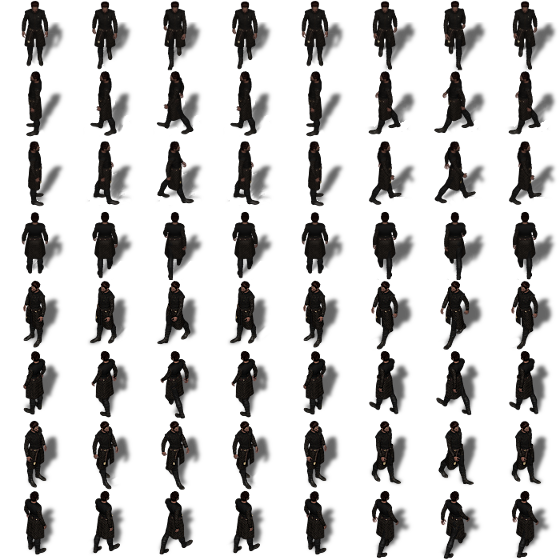
\includegraphics[width=10cm]{8frame_combined}
\caption{Player Spritesheet}\label{fig:knight_sprite}
\end{figure}

Figure \ref{fig:knight_sprite} represents a spritesheet with 8 looped animations
of character motion in 8 directions with 8 frames each. In order to load and use
these animations in the game it is necessary to tell Phaser the frame indices of
each animation and associate every batch with a name. The listing below
demonstrates this procedure:

\lstinputlisting[caption=Sprite Animation Loading]{character_sprite.js}

\subsubsection{Uniform Interface for Input Handling}

The development process becomes increasingly more difficult as the number of
moving parts in the system grows. It also becomes harder to debug and test
individual subsystems in isolated environments and in the case of 'Snowfight'
the development of the game was substantially slowed down by the fact that every
time the page was refreshed, it was necessary to reconnect the controller. In
addition, when some problems appeared it was not clear right away whether the
problem was in the game logic, in the controller code or in the communications
in-between.

One solution to the situation described above was to separate the game from the
controllers and develop it separately by providing the necessary input from the
local keyboard. This way, communication errors and bugs that concern controller
rendering would not stagnate the evolution of the core game.

From the implementation point of view the task required a unified interface for
all possible input sources, in this case only two of them. However, such an
approach opened opportunities to connect an artificial intelligence bot to the
abstract input device, which permits the addition to the game of non-player
characters (NPC) that would be controlled by the computer.

The base class of the Controller sets up the necessary variables and a set of
helper functions like the one in the listing below (\ref{lst:base_controller}),
that performs a check if a button was pressed just before the function call or
it was down all along.

\lstinputlisting[caption=Controller Base Class Highlights, label=lst:base_controller]{controller_base.js}

At the same time, listings \ref{lst:local_controller} and
\ref{lst:remote_controller} contain the specific bits of code that govern input
collection from the local keyboard and a remote mobile device respectively. The
main difference between the two is the fact that a local controller should be
update every iteration of the game loop in order to represent the accurate state
of the input device, while the remote controller is updated asynchronously by
means of callbacks.

\lstinputlisting[caption=Local Controller, label=lst:local_controller]{controller_local.js}

\lstinputlisting[caption=Remote Controller, label=lst:remote_controller]{controller_remote.js}


% \subsubsection{High-Level Game Logic}


\subsection{Controller}

The second major part of the system is the remote controller that is used to
operate a character on the main game screen. Following the motivations described
in the chapter on domain analysis, it represents a web page rather then a native
mobile application. As a result, it requires no prior installation procedures
because any modern mobile device is likely to have a decent web browser that
supports the necessary technological specifications.

The primary goal of the controller component is to provide an experience similar
to using a dedicated gaming device like a gamepad. The touch screen of a mobile
phone can be used to model various control elements like buttons and joysticks.
Even thought these fall short of three-dimensional tactile feedback, they can be
customized and optimized for an engaging and efficient gaming experience.
Moreover, modern browser APIs can trigger device vibrations of different
patterns in order to provide additional feedback.

The design of the controller and the kind of control elements it contains depend
on the type of actions they have to operate. In case of 'Snowfight', there are
two main activities that are controlled by the user, these are \emph{movement}
and \emph{throwing} snowballs. The mechanics of the game state that a snowball
is thrown in the direction of the player's current orientation. This means that
it is not necessary to have a control element like a joystick that would control
the direction, instead, a simple button should be enough to perform this action.
Movement, on the other hand, is a more complex activity and is controlled two
parameters, mainly, direction and speed. An ergonomic solution to this task is a
joystick-like control element. In the context of this system, the element is
called a track ball as it resembles a ball when viewed on the screen.

Figure \ref{fig:gamepad} represents a development version of the web-based
'gamepad' rendered on the screen of a mobile device in landscape mode. The left
side contains the track ball element for movement and the right side has the
button for throwing snowballs. The blue button at the top is a shortcut for
switching to full-screen mode.

\begin{figure}[!h]
\centering
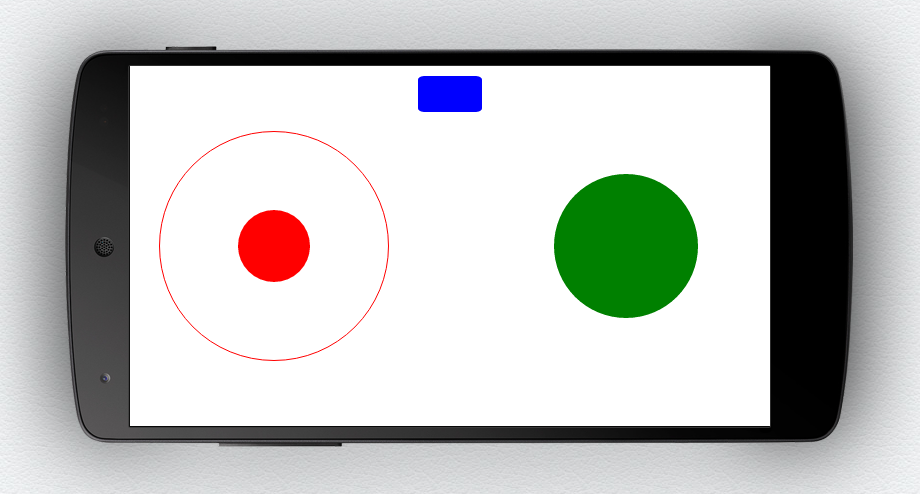
\includegraphics[width=15cm]{gamepad_nexus}
\caption{Web-based Gamepad}\label{fig:gamepad}
\end{figure}

As it is a web application, the controller and its elements are nothing but an
HTML5 document with appropriate styles and some scripts attached. The controller
layout is presented in the listing below. All elements are constructed of
\emph{div} tags that have specific class and id attributes in order to be later
processable by style-sheets and scripts.


\lstinputlisting[language=HTML, caption=HTML Layout of the Controller]{controller.html}

%\subsubsection{Mouse vs Touch Gestures}

\subsubsection{Track Ball Control Element}

In order to control character movement, it is necessary to represent some how
numerically this activity. In its simplest instance, movement on a plane has a
direction and speed, this maps perfectly onto the characteristics of a two-
dimensional vector, specifically its orientation and magnitude. Given a data
model, the next step is to come up with a control element that is able to
generate such data as a result of user input. On conventional gamepads this
feature is attributed to joysticks. They can be tilted to a certain degree
within a range in 2 directions, thus generating a set of 2D coordinates.
Joysticks also include a spring that returns them to the initial position in
case of no user input.

In the context of a touch screen device, it is not that simple to create a
moving stick, however, it is possible to draw a kind of ball that would track
the motion of a finger pressing on the screen and would reset to its initial
position when the touch motion is terminated. In addition, the web browser
interprets touch events in a different way from events generated by a mouse
device. Moreover, complex gestures like \emph{pan}, \emph{pinch zoom},
\emph{rotate} and \emph{swipe} require considerable effort in writing code that
detects these gestures, identifies the right type and fetches appropriate data
sets. Luckily, these problems have been solved by other people who developed
libraries specifically for such tasks. This thesis project makes use of the
HammerJS\cite{hammer} library that can recognize an handle gestures made by
touch, mouse and pointerEvents.

Gesture recognition is easily enabled by creating a \emph{Hammer} object
instance and specifying the HTML element that should trigger the events.

\lstinputlisting[caption=HammerJS Setup, label=lst:hammer]{hammer.js}

Listing \ref{lst:hammer} demonstrates how the ball element is passed to a
\emph{Hammer} object. After that, an option is specified to track \emph{panning}
motion in all direction. The \emph{pan} recognizer generates 3 kinds of events:
\emph{panstart}, \emph{panmove}, \emph{panend}. The listing above also shows how
callbacks are attached to each of the events in order to make use of the
information that is generated by them.


\subsubsection{Button}

The button part of the controller was considerably easier to implement as there
where no gestures involved. However, there was one aspect that had to be
clarified. When a button is pressed, its color should change to give some kind
of feedback to the user. This can be done through CSS pseudo-classes in a
trivial way, but it turns out such an approach has a drawback. There is a delay
of approximately 300ms between clicking on the button and the color change. In
case of usual websites it is almost unnoticeable, however, in case of games,
immediate feedback is crucial and the lack of it impacts severely the user
experience.

A logic workaround to this problem is to trigger the color change through
JavaScript code, by adding or removing the respective CSS class attribute, as it
is shown in listing \ref{lst:button}

\lstinputlisting[caption=Button Color Switch, label=lst:button]{button_color.js}


%\subsubsection{Responsive Design}

\subsection{Peer to Peer Communication}

Communication is the focal point of this thesis and makes all parts of the
system work as a whole. The game and the controller are nothing but simple web
applications and present no special value by themselves. In order to make them
communicate and interact, it is possible to apply several techniques. Most
things on the web communicate under a client-server architecture. This implies
there is an entity (a server) that orchestrates the whole process, it performs
all computations and provides services to the clients who always connect
directly to it. This project, however, has a slightly different twist to it.

The game and the controller are both applications are executed on the client
machine, moreover, there can be many simultaneous game sessions that must not
overlap in terms of communication. If the system were to employ the client-
server architecture, all the communications would have to be proxied through a
main server which would maintain control over all games and controllers.
Obviously, this model would be painfully slow and inefficient as large amounts
of data would have to travel long distances between devices and the server even
though the game computer and all the player are located in the same room and
connected to the same network.

In this context, the best option is a peer-to-peer communication model that
permits the exchange of information between parties directly, without the use of
intermediaries. Modern browser have recently introduced support for the WebRTC
technology that enables peer-to-peer communication with the use of a server only
for establishing the connection.


\subsubsection{Setting Up a Connection with PeerJS}

WebRTC programming interfaces are quite low level and performing the basic tasks
requires considerable effort from the developer. As with other software there
are libraries that have gathered the boilerplate code that is often used in
projects and hide it under simpler and higher level APIs. 'Snowfight' uses
PeerJS\cite{peerjs} which wraps the browser's WebRTC implementation to provide a complete,
configurable, and easy-to-use peer-to-peer connection API. Equipped with nothing
but an ID, a peer can create a P2P data or media stream connection to a remote
peer.

\lstinputlisting[caption=PeerJS Initialization, label=lst:peer_init]{peer_creation.js}

Listing \ref{lst:peer_init} shows how easy it is to initialize a Peer object. It
is enough to provide the address and port of a PeerJS server that will broker
the connections. A data connection is established simply by invoking the
\emph{connect} method on the Peer object. At the same time it is possible to
send arbitrary metadata that will be associated with the connection, in this
case it is the player's name which can be entered by the user. Once a connection
is open, it is trivial to send data over it:

\lstinputlisting[caption=Sending Data Using a 'DataConnection' Object]{peer_send.js}

When a controller initiates a peer-to-peer connection, the game lobby has to
catch this event and execute the necessary procedures in order to be able to
receive data. As many other things in JavaScript this is done by the use of
callbacks that are attached to specific events. Listing \ref{lst:peer_hub_init}
shows that every incoming connection object, that is intercepted by the game
while in lobby, is collected in a JavaScript array.

\lstinputlisting[caption=Connection Gathering, label=lst:peer_hub_init]{peer_hub_create.js}

Later on, at the initialization step of the game, every connection is attached
to a \emph{RemoteController} object, which in turn, sets callbacks (listing
\ref{lst:controller_callbacks}) that process incoming data and update the
internal state of the controller.

\lstinputlisting[caption=Controller Callbacks, label=lst:controller_callbacks]{controller_callbacks.js}


\subsubsection{Communication Protocol}

Establishing a connection is definitely not enough for an efficient and fruitful
communication. The chosen format of data that is to be exchanged between the
parties can heavily influence the flexibility and the performance of the system.
Devising a protocol is not a simple task because there are a lot of questions
that a developer should be able to answer before proceeding to the
implementation step.

Some of the things that should be clarified are listed below:

\begin{itemize}
\item what kind of data to transmit;
\item how to order the data inside of a message;
\item how to encode the transmission;
\item how reliable should be the connection.
\end{itemize}

The fact that a communication library is being used, greatly simplifies some of
the aspects of the protocol. For instance, PeerJS by default encodes all
messages in binary be it a string or a JavaScript object. The gaming context
also emphasizes performance over reliability, that is, if a message about the
current position of the trackball is lost, nothing catastrophic will happen.

The question that remains, though, is what kind of data should be sent from the
controller to the game and how should a message be formatted. At this point in
development, the system needs only two types of messages, one about the
trackball position changes and one about the changes in the state of a button.
These to types can be easily differentiated by a \emph{type} field in the top
level object of the message. In addition, a small number of message types does
not enforce a deeply nested structure. Listings \ref{lst:trackball_msg} and
\ref{lst:button_msg} represent examples of messages for trackball position
change and a button event respectively:

\lstinputlisting[caption=Trackball Message, label=lst:trackball_msg]{trackball_msg.json}

\lstinputlisting[caption=Button Message, label=lst:button_msg]{button_msg.json}

This protocol is by far not the best and the most efficient, but it works fine
for the current state of the system. At the same time, in case of further
development, it is certain that the message format will change drastically.

\subsection{Implementation Conclusions}

This chapter of the thesis gave an overview of the tools and techniques used
build all the parts of the system. It presented the Phaser framework and a
typical structure of a game that uses this framework. The sections about the
controller explained the motivation behind its components and control elements.
The final sections on peer-to-peer communication described the procedures that
where employed in order to establish a communication channel between the
controller and the main game. It also provided a brief description of the
protocol used to exchange information and control messages between the parties.

Overall, the technical side of the project is relatively straight forward and
does not contain scientific breakthroughs nor great innovations. On the other
hand, it represents an attempt to realize an already existing concept and
identify various pattern that can be reused in other projects on a greater and
more innovative scale.

\clearpage
